%%% LaTeX Template: Two column article
%%%
%%% Source: http://www.howtotex.com/
%%% Feel free to distribute this template, but please keep to referal to http://www.howtotex.com/ here.
%%% Date: February 2011

%%% Preamble
\documentclass[	DIV=calc,%
							paper=a4,%
							fontsize=12pt,%
							onecolumn]{scrartcl}	 					% KOMA-article class

\usepackage{lipsum}													% Package to create dummy text
\usepackage[brazil]{babel}										% English language/hyphenation
\usepackage[protrusion=true,expansion=true]{microtype}				% Better typography
\usepackage{amsmath,amsfonts,amsthm}					% Math packages
\usepackage[pdftex]{graphicx}									% Enable pdflatex
\usepackage[svgnames]{xcolor}									% Enabling colors by their 'svgnames'
\usepackage[hang, small,labelfont=bf,up,textfont=it,up]{caption}	% Custom captions under/above floats
\usepackage{epstopdf}												% Converts .eps to .pdf
\usepackage{subfig}													% Subfigures
\usepackage{booktabs}												% Nicer tables
\usepackage{fix-cm}													% Custom fontsizes
\usepackage[utf8]{inputenc}
\usepackage[top=2.5cm, bottom=2.5cm, left=2.5cm, right=2.5cm]{geometry}
\usepackage[ddmmyyyy]{datetime}
\addto\captionsenglish{%
	\renewcommand\tablename{Tabela}
	\renewcommand\figurename{Figura}
} 
 

 
%%% Custom sectioning (sectsty package)
\usepackage{sectsty}													% Custom sectioning (see below)
\allsectionsfont{%															% Change font of al section commands
	\usefont{OT1}{phv}{b}{n}%										% bch-b-n: CharterBT-Bold font
	}

\sectionfont{%																% Change font of \section command
	\usefont{OT1}{phv}{b}{n}%										% bch-b-n: CharterBT-Bold font
	}



%%% Headers and footers
\usepackage{fancyhdr}												% Needed to define custom headers/footers
	\pagestyle{fancy}														% Enabling the custom headers/footers
\usepackage{lastpage}	

% Header (empty)
\lhead{}
\chead{}
\rhead{}
% Footer (you may change this to your own needs)

%% ====================================
%% ====================================
%% mude o rodape  do projeto
%% ====================================
%% ====================================

\lfoot{\footnotesize \texttt{Cabeamento estruturado} \textbullet ~Projeto de Infraestrutura de Redes - APS Engenharia}


\cfoot{}
\rfoot{\footnotesize página \thepage\ de \pageref{LastPage}}	% "Page 1 of 2"
\renewcommand{\headrulewidth}{0.0pt}
\renewcommand{\footrulewidth}{0.4pt}



%%% Creating an initial of the very first character of the content
\usepackage{lettrine}
\newcommand{\initial}[1]{%
     \lettrine[lines=3,lhang=0.3,nindent=0em]{
     				\color{DarkGoldenrod}
     				{\textsf{#1}}}{}}



%%% Title, author and date metadata
\usepackage{titling}															% For custom titles

\newcommand{\HorRule}{\color{DarkGoldenrod}%			% Creating a horizontal rule
									  	\rule{\linewidth}{1pt}%
										}

\pretitle{\vspace{-10pt} \begin{flushleft} \HorRule 
				\fontsize{40}{40} \usefont{OT1}{phv}{b}{n} \color{DarkRed} \selectfont 
				}

%% ====================================
%% ====================================
%% mude o titulo  do projeto
%% ====================================
%% ====================================

\title{Projeto de Infraestrutura de Rede de Dados - APS Engenharia}					% Title of your article goes here

%% ====================================



\posttitle{\par\end{flushleft}\vskip 0.5em}

\preauthor{\begin{flushleft}
					\large \lineskip 0.5em \usefont{OT1}{phv}{b}{sl} \color{DarkRed}}
\author{Anderson Pacheco dos Santos }  	% Author name goes here


\postauthor{\footnotesize \usefont{OT1}{phv}{m}{sl} \color{Black} 
					\\Universidade Tecnológica Federal do Paraná - Câmpus Cornélio Procópio 								% Institution of author
					\par\end{flushleft}\HorRule}

\date{}																				% No date




%%% Begin document
\begin{document}
\maketitle
\thispagestyle{fancy} 	
\thispagestyle{empty}		% Enabling the custom headers/footers for the first page 
% The first character should be within \initial{}




%% ====================================
%% ====================================
%% mude o resumo  do projeto
%% ====================================
%% ====================================

\initial{O}\textbf{presente projeto destina-se ao planejamento da implantação simulada da infraestrutura da rede de comunicação de dados da empresa fictícia APS Engenharia. Para tanto, tem-se a premissa de que o edifício encontra-se incorporado, no entanto, não possui elementos de infraestrutura adequados para a instalação de componentes de rede. O presente estudo irá definir um novo projeto de redes para a empresa, observando os passivos que serão empregados, a fim de garantir o plano de certificação. Com o levantamento da planta física da edificação, será executado o levando de custos e quantidade de materiais, bem como da terceirização de serviços de instalação de condutores externos, haja vista o prédio não possuir tal elemento de infraestrutura. Constituirá o corrente documento, informações sobre os procedimentos de manutenção após a implantação. Registra-se ainda que a empresa torna-se diretamente dependente da rede de comunicação de dados, uma vez que, todas as ferramentas de software e armazenamento de dados da empresa estão diretamente ligados aos serviços de cloud computing.}


%% ====================================
\begin{figure}
	\centering
	
\includegraphics{utfpr}
\end{figure}

\vspace{2cm}
\centerline{\textit{\textbf{\today}}}

\clearpage
    \renewcommand*\listfigurename{Lista de figuras}
\listoffigures

\renewcommand*\listtablename{Lista de tabelas}
\listoftables




\clearpage
\renewcommand{\contentsname}{Sumário}
\tableofcontents
\clearpage

%% ====================================
%% ====================================
%% Inicio do texto
%% ====================================
%% ====================================
\section{Introdução}
Explique nesta primeira seção qual seria o perfil do caso. Perfil do cliente, quantidade de colaboradores, quantidade de equipamentos de TI atualmente.

Indique também nesta seção o escopo do projeto.

Apresente um overview do parque tecnológico do caso.
\subsection{Benefícios}
Explique quais seriam os benefícios provenientes após a execução deste projeto.

\subsection{Organizações Envolvidas}
Coloque o nome de todas as organizações envolvidas. Se for um projeto real, identifique quais as responsabilidades de cada uma das organizações. É comum que em um projeto de redes (cabeamento), temos várias organizações, sendo que cada uma delas com uma determinada responsabilidade.

Sugestão: crie uma tabela contento a relação delas.



\section{Estado atual}
Aprente o estado atual da rede. Caso não tenha rede, desconsiderar esta seção.

Caso tenha rede, deixe claro:
\begin{itemize}
	\item os passivos de rede atuais:path panels, cabos, etc..;
	\item as principais reclamações dos usuários. Qual o principal motivo da reestruturação? Efetue uma pesquisa junto aos colaboradores para determinar quais problemas a rede apresenta.
	\item Observações. Analise a rede e verifique se há estruturas que não se enquadram nas normas ou que indicam suspeita de problemas.
\end{itemize}

\section{Requisitos}
Crie uma enumeração dos requisitos do projeto.

\section{Usuários e Aplicativos}

\subsection{Usuários}
A empresa possui 21 colaboradores, sendo que 19 são usuários ativos do parque de informática da entidade.
Os usuários em sua maioria exercem funções exclusivamente administrativas e em geral possuem conhecimentos amplos para utilização dos recursos tecnológicos disponíveis, sendo atendidos por um colaborador que exerce a função de suporte e é responsável pelos ativos e passivos da estrutura tecnológica da empresa. Este por sua vez, possui formação acadêmica na área de ciências da computação.
Existe a perspectiva de crescimento de 20 porcento no quadro de colaboradores para os próximos 3 anos.

\subsection{Aplicativos}
As ferramentas e serviços utilizados na unidade encontram-se em sua maioria na nuvem, tornando esse o principal e mais importante ponto crítico a ser considerado nesse projeto. Os usuários utilizam o Domínio de rede para login nas estações de trabalho o qual é validado em LDAP remoto, utilizam sistemas de Intranet, provedor de e-mail próprio, ferramentas e softwares remotos, armazenamento de arquivos em servidor externo (NAS), acesso a internet com permissões de servidores de proxy e firewall remotos, entre outros.


\section{Estrutura predial existente}


%inicio dos comandos para criar uma nova pagina A3 vertical
\clearpage
\KOMAoptions{paper=a3, paper=portrait, DIV=15}
\recalctypearea


\begin{figure}
	%	\centering
	\noindent\makebox[\textwidth][c]{
		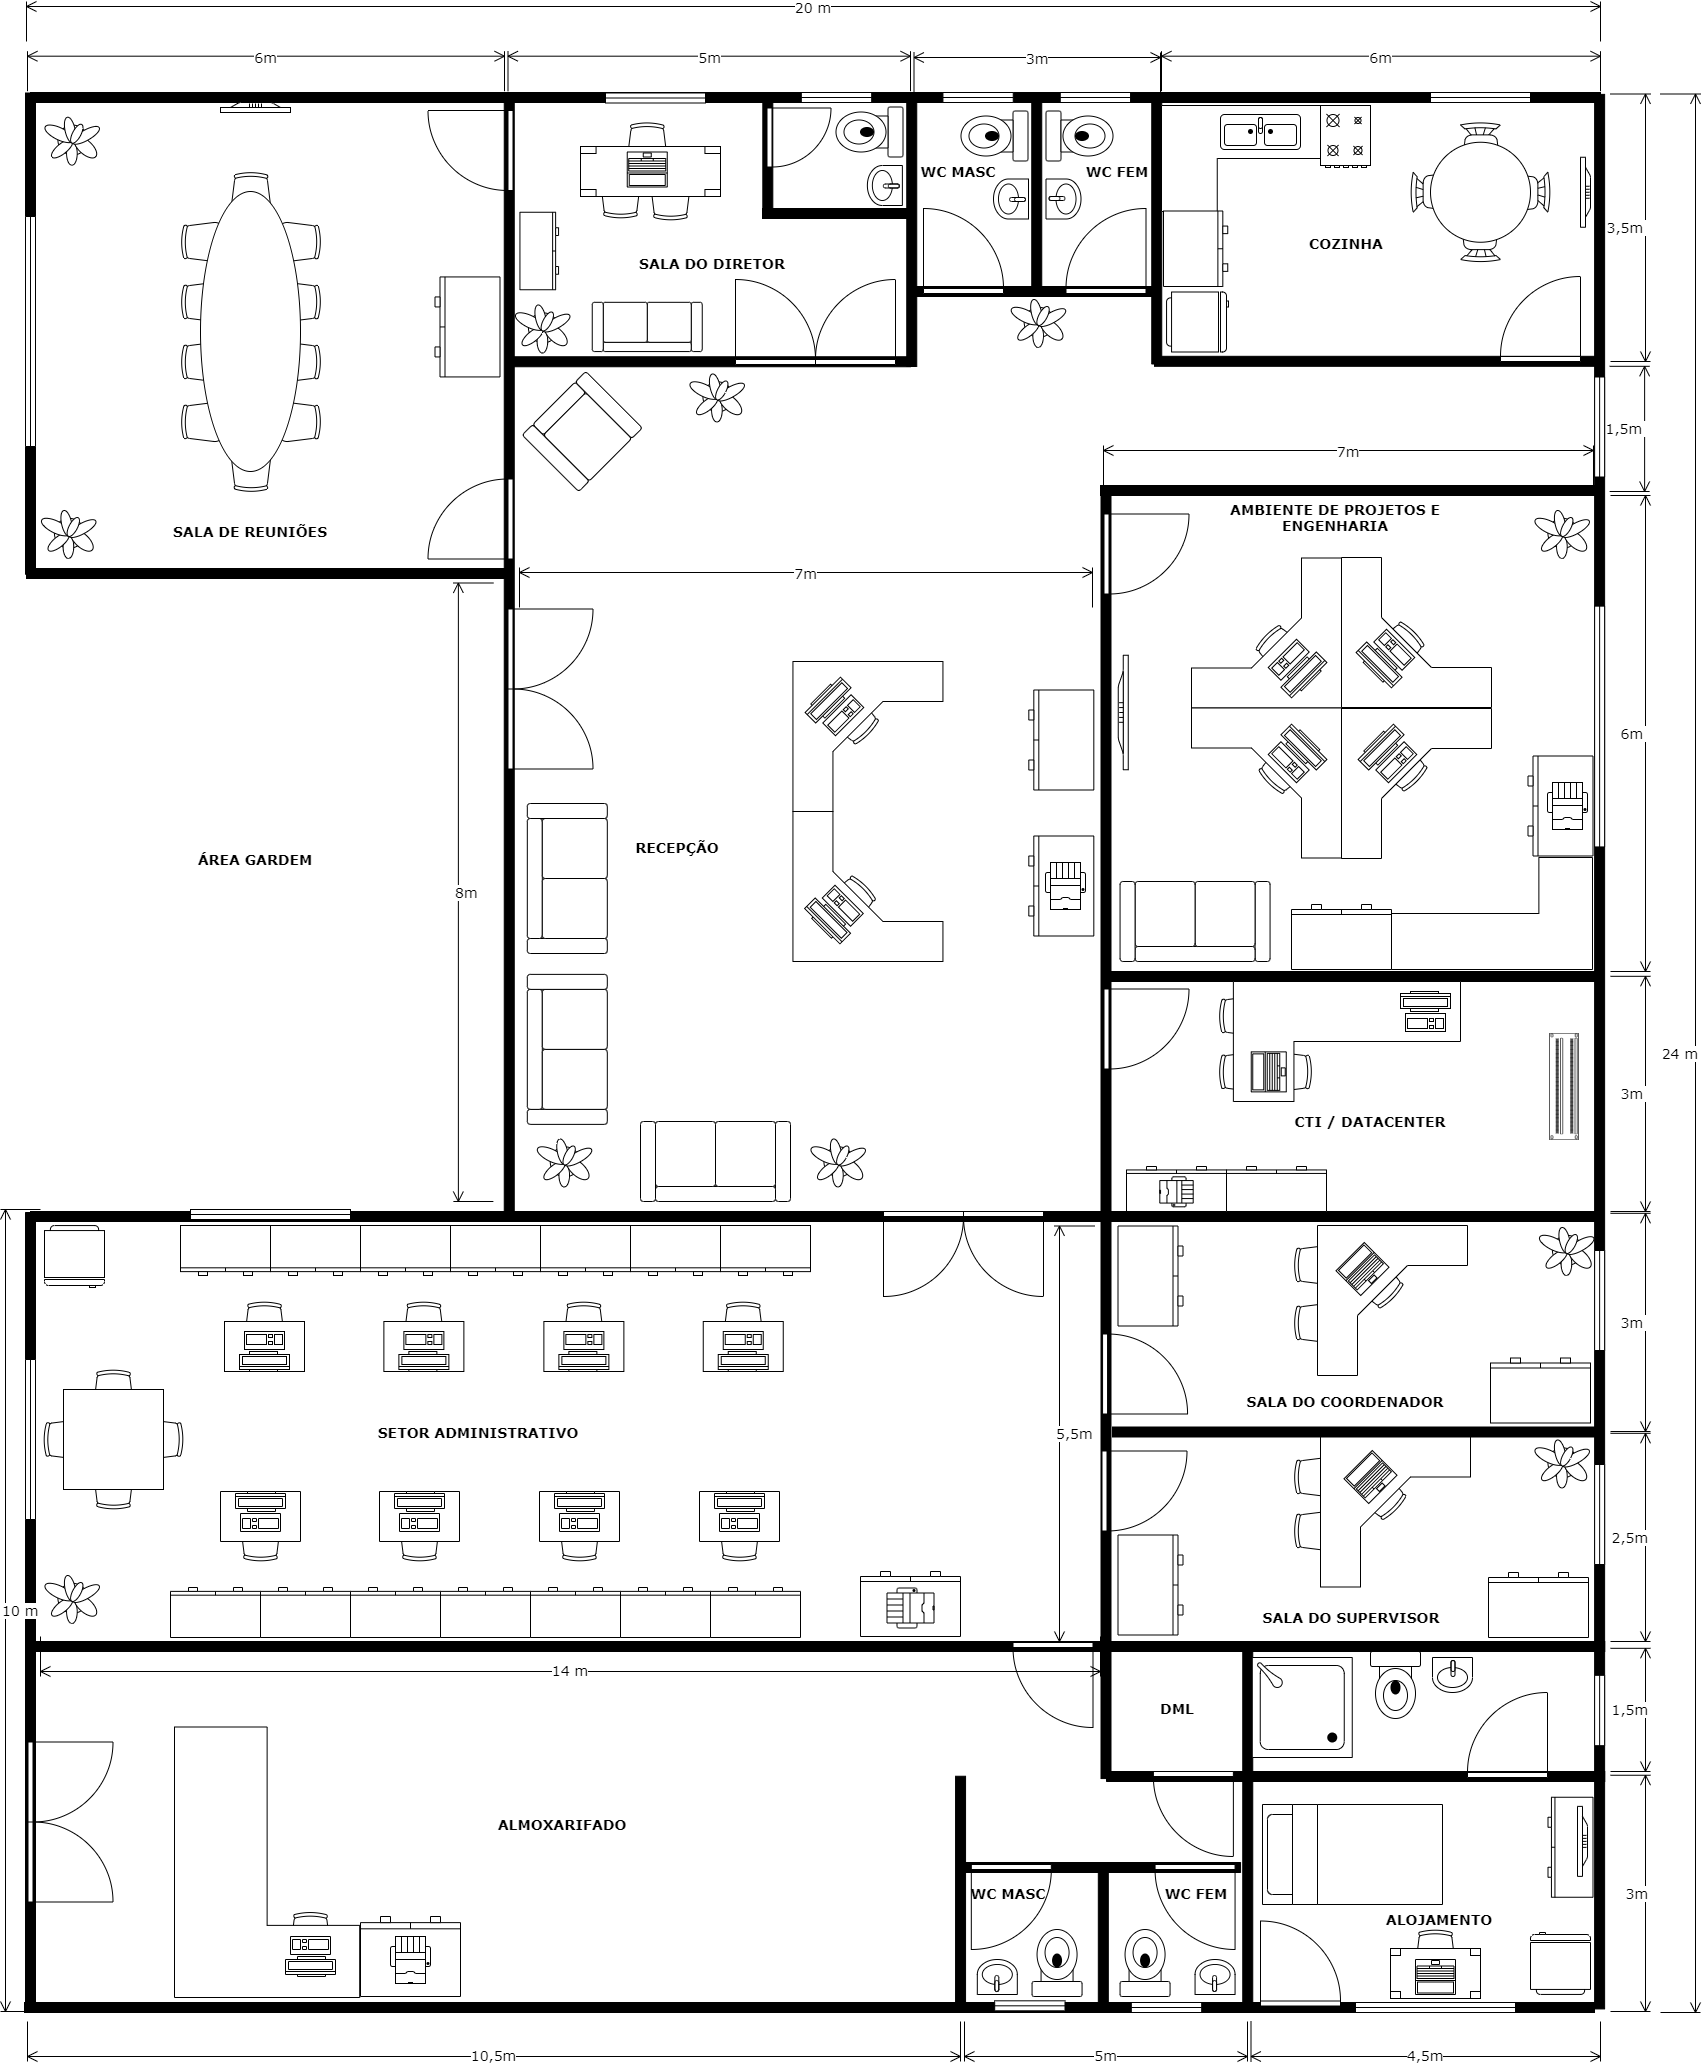
\includegraphics[height=\textheight]{plantabaixa}
	}
	\caption{Planta Baixa do Edifício da Empresa APS Engenharia.}
	\label{plantabaixa}
\end{figure}

%Retornar ao formato A4
\clearpage
\KOMAoptions{paper=a4, paper=portrait, DIV=15}
\recalctypearea
%-- reinicio em A4 


\section{Planta Lógica - Elementos estruturados}

\subsection{Estado atual}


%inicio dos comandos para criar uma nova pagina A3 vertical
\clearpage
\KOMAoptions{paper=a3, paper=portrait, DIV=15}
\recalctypearea


\begin{figure}
	%	\centering
	\noindent\makebox[\textwidth][c]{
		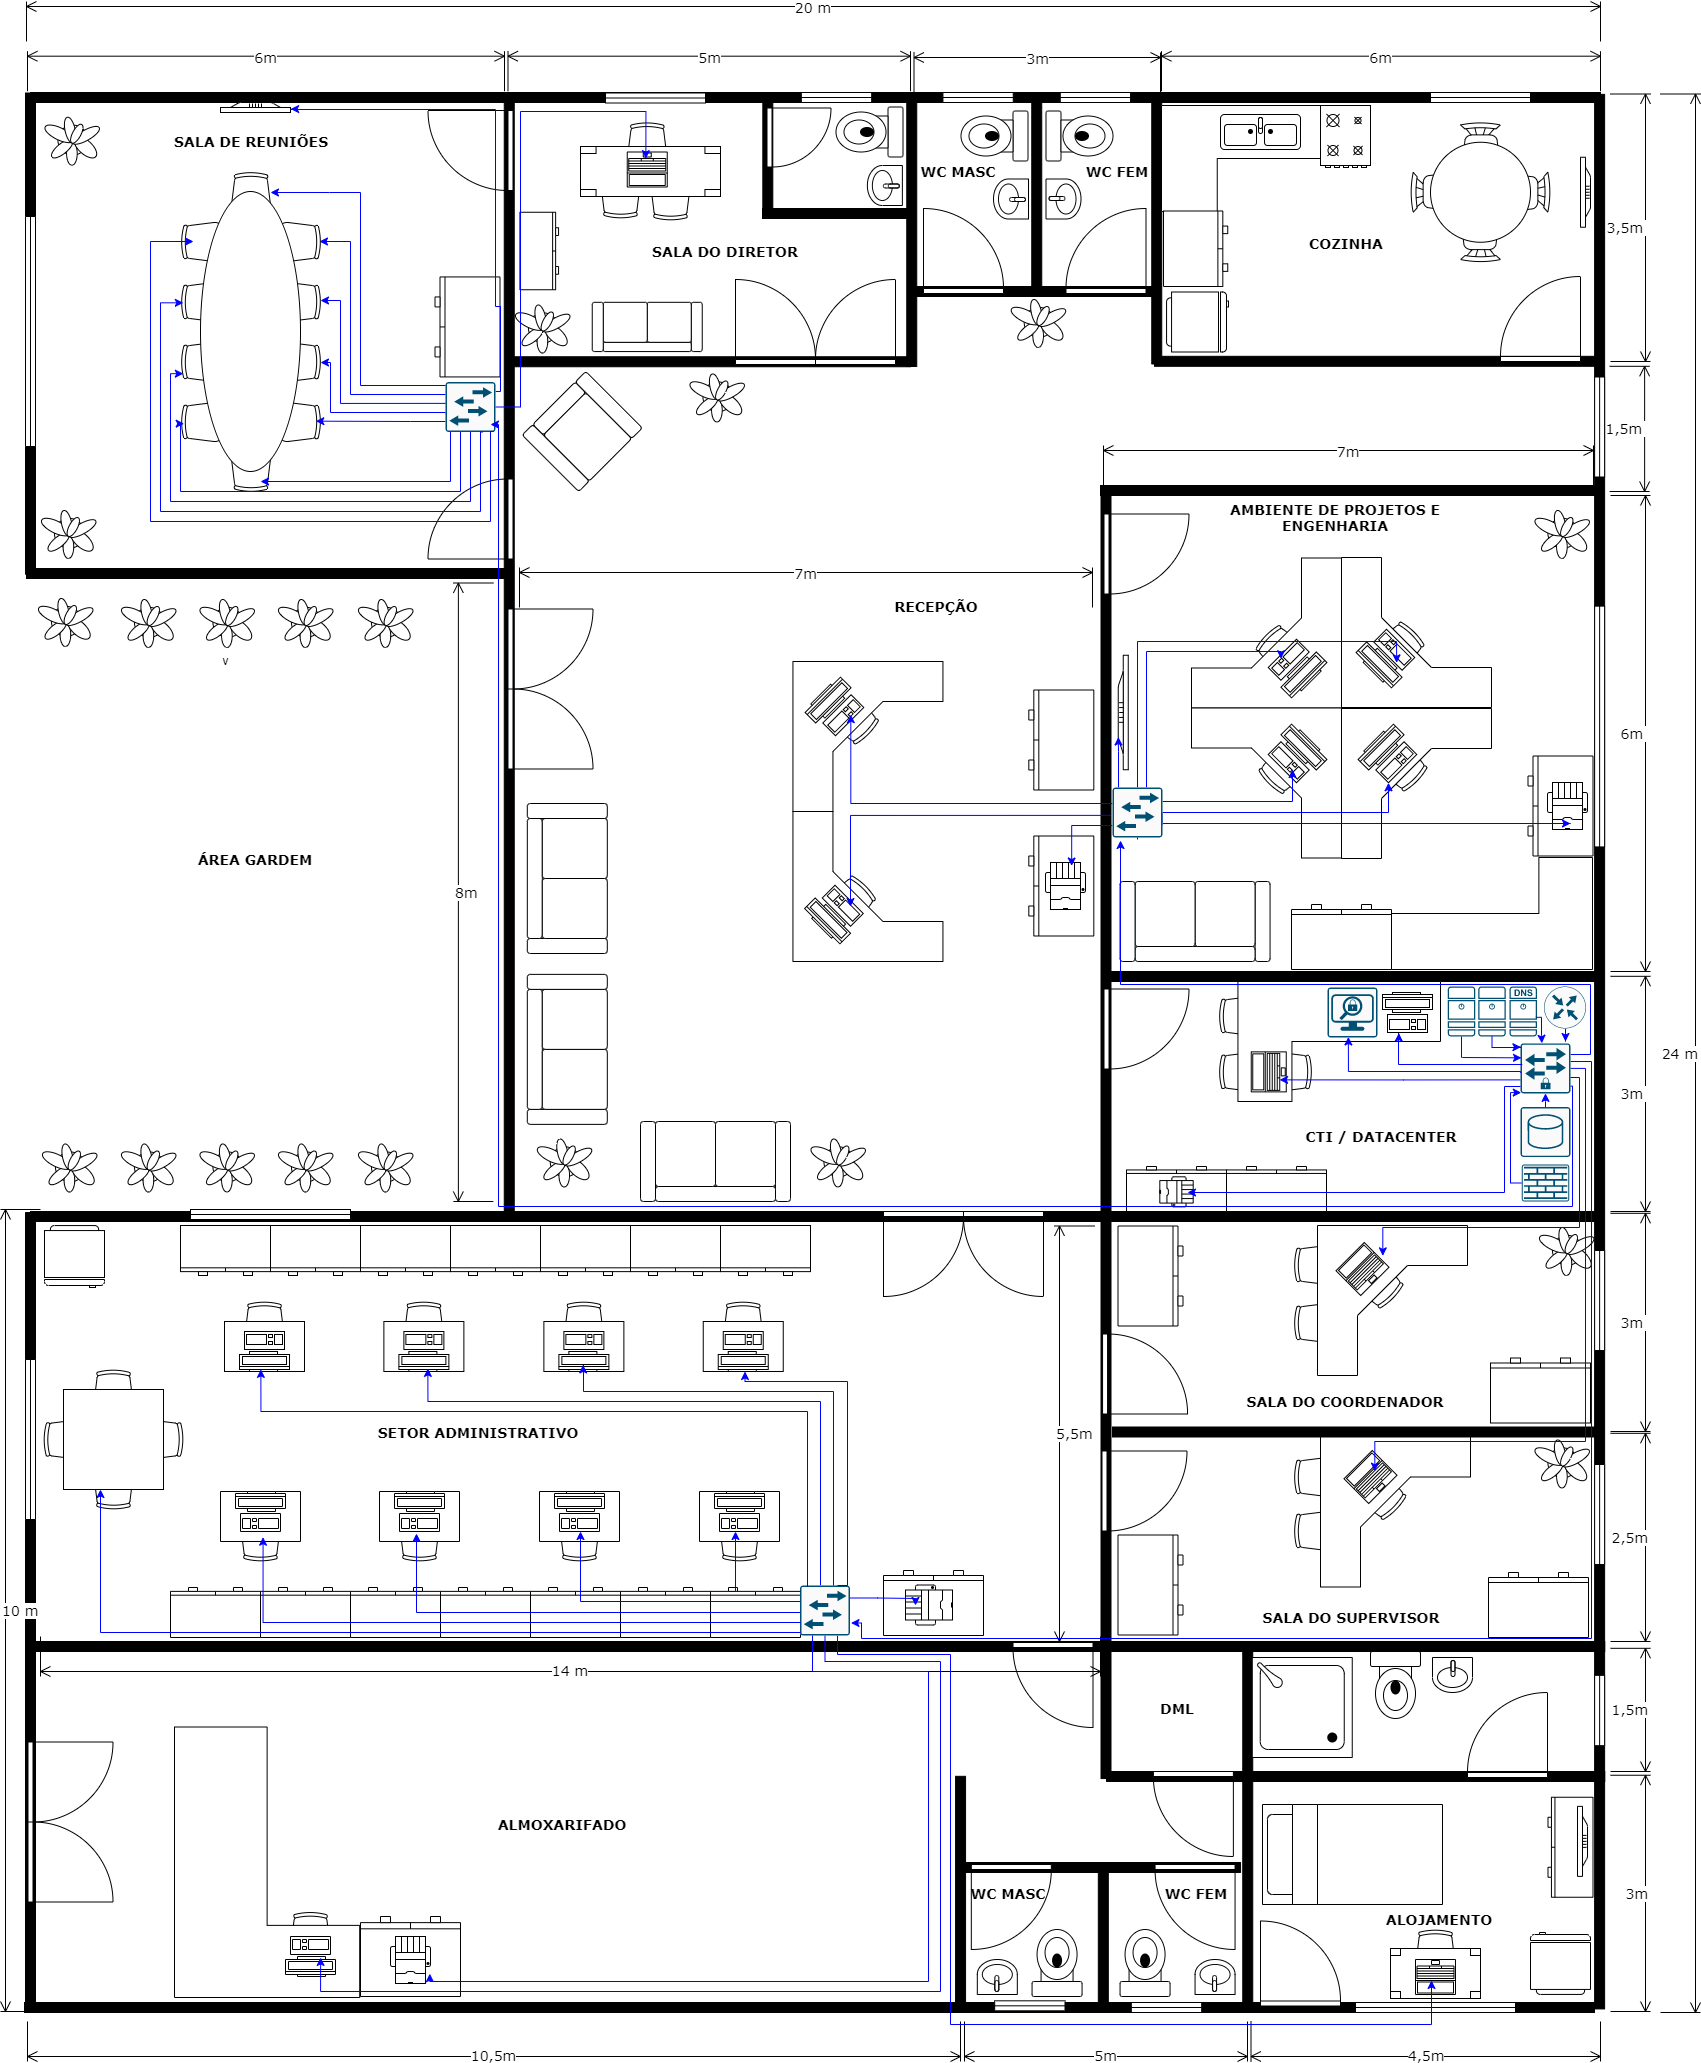
\includegraphics[height=\textheight]{plantalogica.png}
	}
	\caption{Planta Lógica do Edifício da Empresa APS Engenharia.}
	\label{plantalogica}
\end{figure}

%Retornar ao formato A4
\clearpage
\KOMAoptions{paper=a4, paper=portrait, DIV=15}
\recalctypearea
%-- reinicio em A4 


\subsection{Topologia}
Proposta futura, proposta após implantação.
Deve conter o diagrama da rede. Atente-se a redundância  e ligações truncadas.
Deve explicar todos termos e componentes utilizados nestas plantas. Por exemplo: entrance facility, work area, horizontal cabling, etc..

Todos os elementos das figuras devem ser explicados. 
Crie esboço da configuração dos racks e brackets. Explique cada um dos componentes. Você pode criar uma tabela contendo figuras dentro, ou criar uma tabela e incluí-la como imagem. Por exemplo, verifique a tabela \ref{tab1}.

\begin{table}[h!]
\centering
\caption{Exemplo de tabela explicativa}
\label{tab1}
\begin{tabular}{|l|l|l|}
\hline
\multicolumn{3}{|l|}{Figura na Tabela} \\ \hline
1        & Rack          & \includegraphics[scale=0.2]{fig1}        \\ \hline
2        & Rack 2        & \includegraphics[scale=0.2]{fig1}        \\ \hline
\end{tabular}
\end{table}

\subsection{Encaminhamento}
Eletrodutos, calhas, e qualquer material em que os cabos serão alojados/alocados.

\subsection{Memorial descritivo}
\begin{table}[]
	\centering
	\caption{Descrição dos elementos passivos do projeto}
	\label{tab_passivos}
	\begin{tabular}{|l|c|c|c|}
		\hline
		\textbf{ELEMENTO PASSIVO}  & \textbf{QUANTIDADE} & \textbf{MEDIDA} & \textbf{FABRICANTE} \\ \hline
		Rack Padrão Piso 32u       & 1                   & un              & Saint Blanc         \\ \hline
		Patch Panel 24 Portas Cat6 & 2                   & un              & Furukawa            \\ \hline
		Patch Cords Cat 6 - 1m     & 20                  & un              & Furukawa            \\ \hline
		Patch Cords Cat 6 - 2m     & 20                  & un              & Furukawa            \\ \hline
		Cabo UTP Cat 6             & 966                 & m               & Furukawa            \\ \hline
		Tomadas para embutir RJ45  & 40                  & un              & Enerbras            \\ \hline
		Eletroduto 2"              & 98,5                & m               & Tigre               \\ \hline
		Eletroduto 1.1/4"          & 100                 & m               & Tigre               \\ \hline
		Fita Hellerman 230mm       & 200                 & un              & Tyton               \\ \hline
		Régua de energia 1u        & 2                   & un              & Fiolux              \\ \hline
		Régua organizadora 1u      & 2                   & un              & Pier Telecom        \\ \hline
		Bandejas para Rack 2u      & 3                   & un              & Cwb Metal           \\ \hline
	\end{tabular}
\end{table}
Relacione todos os equipamentos passivos que serão utilizados, tipo, fabricante, quantidade.



\subsection{Identificação dos cabos}
Explique como os cabos serão identificados em seu projeto. Coloque uma relação dos cabos instalados e identificados.

\section{Implantação}
Estabeleça um cronograma de implantação:
Remoção de equipamentos existentes (destino para descarte), instalação dos condutores, instalação dos cabos, 
identificação dos cabos, montagem dos racks, certificação, etc... Crie atividades e estabeleça o tempo de execução. Se for um projeto real, indique também quais os responsáveis pela execução do projeto e de cada uma das etapas.

Defina marcas (e padrões) e fornecedores se for o caso. Atenção a contratados e subcontratados para a realização das atividades. Estabeleça a responsabilidade de execução da atividade e também da validação dela.

Utilize algum software para gerear o cronograma. Excel,etc. O fundamental é dividir em etapas, descrever e estimar o tempo de cada uma delas.

Segue uma relação de ferramentas:
http://asana.com/, 
https://trello.com/, 
http://www.ganttproject.biz/, 
http://www.orangescrum.org/. 

\section{Plano de certificação}
Quais seriam as etapas para a certificação? 
Quais os locais e horários para execução da certificação na rede? Toda rede será certificada?
Como os testes seriam executados?
Quais relatórios de certificação serão (ou deveriam ser) entregues? 

\section{Plano de manutenção}

Revisões periódicas na rede, emissão de certificados para novos pontos.

\subsection{Plano de expansão}
Existe um plano de expansão? Quantos novos pontos poderão ser acrecidos na rede, antes de migração de equipamentos na camada 2? Se houver expansão, quais equipamentos deverão ser direcionados para as estremidades da rede? 

\section{Risco}
Enumerar e explicar os riscos do projeto.

\section{Orçamento}
Crie uma relação de orçamentos baseado na seções anteriores.

\section{Recomendações}
Observações e recomendações para o cliente.

\section{Referências bibliográficas}
Utilize o mendley, o jabref ou diretamente o bibtex para gerenciar suas referências biliográficas. As referências são criadas automaticamente de acordo com o uso no texto.

Exemplo: Redes de computadores, segundo \cite{t2013} é considerada..... Já \cite{kurose2010} apresenta uma versão...

Analisando os pressupostos de \cite{ref3} e \cite{ref4} concluimos que....


\renewcommand\refname{} %%Referências bibliográficas}  
\bibliographystyle{ieeetr}
\bibliography{referencias}  


\end{document}